\chapter{Réseaux de neurones}

\section{Apprentissage automatique}

Avant de parler de neurones et de réseaux de neurones, nous commencerons par rappeler rapidement ce qu'est l'apprentissage automatique, ses différentes formes et fixerons certaines notations pour la suite de ce document.

L'apprentissage automatique au sens général peut être défini comme un processus permettant à une machine d'évoluer afin de résoudre une tâche ou un problème. Il en existe plusieurs formes parmi lesquelles l'apprentissage supervisé, l'apprentissage non-supervisé et l'apprentissage par renforcement.

L'apprentissage supervisé est celui qui nous intéressera le plus, il sera donc davantage détaillé. Dans un problème d'apprentissage il est donné un ensemble de taille finie $N$ de couples d'entrée, sortie que nous noterons 

\centerline{$(x^{(1)},y^{(1)}),..., (x^{(N)}, y^{(N)})$}

Ces couples sont appelés exemples. Les entrées proviennent d'un espace $\mathcal{X}$ de dimension $n$ et les sorties d'un espace $\mathcal{Y}$ de dimension $m$. Une hypothèse classique de l'apprentissage automatique est de supposer que les entrées sont générées de manière indépendante selon une certaine loi de probabilité sur $\mathcal{X}$. Plus formellement, les $(x^{(i)})_{i \in \{1, ..., N\}}$ sont les réalisations de variables aléatoires $(X_i)_{i \in \{1, ..., N\}}$ avec les $X_i$ indépendantes et identiquement distribuées selon une probabilité $p$. Pour plus de commodités, notons $X = \{x^{(i)}, \forall i \in \{1, ..., N\}\}$ et $Y = \{y^{(i)}, \forall i \in \{1, ..., N\}\}$.

L'objectif de l'apprentissage supervisé est alors de découvrir le processus générateur des sorties à partir des entrées. Si ce processus est déterministe, il s'agira d'une fonction $f$ générant les sorties à partir des entrées. L'objectif de l'apprentissage sera donc de trouver à partir des exemples un modèle $\hat{f}$ proche de f. Si le processus est non déterministe, il s'agira alors de retrouver la loi de $p(y|x)$.

Si les sorties prennent leurs valeurs dans un espace $\mathcal{Y}$ infini, le problème est dit de régression. Dans le cas contraire, on parle de problème de classification. Par convention, on choisit les valeurs des classes telles que $\mathcal{Y} = \{0, ..., M-1\}$ avec $M$ le nombre de classes. Si $M = 2$, il s'agit de classification binaire.

Quelque soit le type de problème à résoudre, l'objectif est toujours de trouver une fonction ou une distribution de probabilité proche de celle générant les sorties. Cependant, cette notion de "proche" est très relative. 

\begin{definition}[Erreur sur un exemple]
Soit $e : \mathbb{R}^m \times \mathbb{R}^m \rightarrow \mathbb{R}$ la mesure de performance sur un exemple.
\end{definition}
$e(y, \hat{f}(x))$ représentera l'écart de notre modèle avec la sortie attendue. 

\begin{example}[Erreur quadratique]
Une mesure courante est l'erreur quadratique $e(x, y) \mapsto \Vert x - y \Vert_2^2$.
\end{example}

On définit alors l'erreur sur l'ensemble des exemples :

\begin{definition}[Erreur empirique]
$$
E_{in} = \frac{1}{N}\sum_{i=1}^{N}{e(y^{(i)}, f(x^{(i)})} = \mathbb{E}_{x, y \sim \hat{p}_{data}}(e(y, f(x)))
$$
avec $\hat{p}_{data}$ est la distribution empirique dans l'ensemble des exemples.
\end{definition}

Et l'erreur dans l'absolu, sur toutes les valeurs possibles :

\begin{definition}[Erreur absolue]
$$
E_{out} = \mathbb{E}_{x, y \sim p}(e(y, f(x)))
$$
avec $p$ la distribution réelle des entrées et des sorties.
\end{definition}

L'objectif d'être proche peut alors se traduire par la minimisation de $E_{out}$. Or l'estimation de $E_{out}$ nécessite de connaître $p(x, y)$ pour tout $(x, y)$ dans $\mathcal{X} \times \mathcal{Y}$, ce qui est généralement impossible. Cependant, il est aisé de calculer $E_{in}$, qui est une estimation de $E_{out}$ sur les données disponibles. 

En effet, on a la proposition suivante :
\begin{proposition}
$E_{in}$ est un estimateur non biaisé de $E_{out}$.
\end{proposition}

\begin{proof}
$$
\mathbb{E}_{(x_1, y_1),..., (x_N, y_N) \sim p}(E_{in}) = \frac{1}{N}\sum_{i=1}^{N}{\mathbb{E}_{(x_i, y_i) \sim p}(e(y^{(i)}, f(x^{(i)}))} = \mathbb{E}_{x, y \sim p}(e(y, f(x)))
$$
\end{proof}

Malheureusement, les exemples servant à calculer $E_{in}$ seraient les mêmes que ceux utilisés pour choisir notre modèle. Par conséquent, le modèle serait choisi pour bien fonctionner sur ces exemples. $E_{in}$ sous-estimerait la valeur réelle de $E_{out}$ et ne serait plus un bon proxy pour $E_{out}$.

Une solution simple pour régler ce problème est de découper nos exemples en deux ensembles distincts : l'ensemble d'apprentissage et l'ensemble de test que nous noterons respectivement $(X_{train}, Y_{train})$ et $(X_{test}, Y_{test})$. Nous aurons alors :

\begin{equation}
E_{train} = \frac{1}{N_{train}}\sum_{i=1}^{N_{train}}{e(y^{(i)}_{train}, f(x^{(i)}_{train}))}
\end{equation}

qui servira pour entraîner le modèle pendant l'étape d'apprentissage et :

\begin{equation}
E_{test} = \frac{1}{N_{test}}\sum_{i=1}^{N_{test}}{e(y^{(i)}_{test}, f(x^{(i)}_{test}))}
\end{equation}

qui servira comme proxy de $E_{out}$ et qui permettra d'estimer si notre modèle se généralise bien à des données inconnues.

Nous utiliserons cette dernière solution dans la suite du document. Finalement il est à noter que nous parlerons indifféremment de fonction d'erreur ou de fonction de coût.

\section{Inspiration biologique}
C'est à partir de l'hypothèse selon laquelle le comportement intelligent humain est le résultat de la structure et des éléments de bases du système nerveux central, que l’on a développé les réseaux de neurones artificiels. A la suite des observations biologiques, les scientifiques ont schématisé un neurone en trois parties : les dendrites qui constituent les entrées de l’information créée par un stimulus, un corps où l’information est traitée, et l’axone qui représente la voie de sortie de l’information vers d’autres neurones. Les synapses permettent le contact entre deux neurones, chacun d'entre eux intégrant en permanence jusqu'à un millier de signaux synaptiques. Ces signaux n'opèrent pas de manière linéaire : il y a un effet de seuil. 
Les réseaux de neurones artificiels ont été développés à partir de cette vision et leur but est de modéliser le mécanisme d'apprentissage et de traitement de l'information qui se produit dans le cerveau humain.

\begin{figure}[h!]
\begin{center}
	{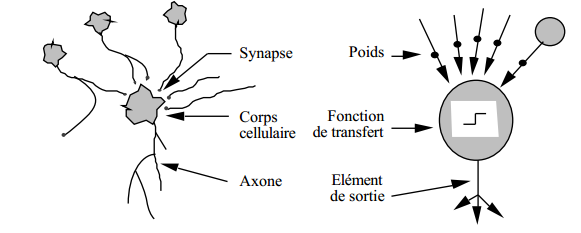
\includegraphics[scale=0.4]{images/chapter1/neurone_bio.png}\label{neurone}}
  \caption{Conception d'un neurone artificiel à partir d'un neurone biologique \\ Source : \textit{Les réseaux de neurones artificiels, Introduction au connexionnisme, Claude Touzet}}
\end{center}
\end{figure}

\section{Un neurone}

\begin{definition}[Neurone]
Un neurone est modélisé par une fonction $f$ de $\mathbb{R}^n$ dans $\mathbb{R}$. Elle est déterminée par trois paramètres : un vecteur de poids $w \in \mathbb{R}^n$, un biais $b \in \mathbb{R}$ et une fonction d'activation $g$. La fonction $f$ se réécrit alors :

\begin{equation}
\forall x \in \mathbb{R}^n, y = f(x) = g(w^Tx+b) = g(\sum_{i=1}^{n}{w_ix_i}+b)
\label{sortie_neurone1}
\end{equation}
\end{definition}

\begin{remark}
Il est usuel de rajouter une composante $x_0$ égale à 1 à chaque entrée afin de pouvoir considérer le biais comme un simple poids. Avec cette convention, la formule \ref{sortie_neurone1} devient :

\begin{equation}
\forall x \in \mathbb{R}^n, y = f(x) = g(w^Tx) = g(\sum_{i=0}^{n}{w_ix_i})
\label{sortie_neurone2}
\end{equation}
\end{remark}

L'analogie avec le neurone biologique est ici claire. La fonction prend plusieurs entrées que l'on peut assimiler aux dendrites, les pondère et renvoie une sortie scalaire qui correspond à l'axone.

La figure \ref{neurone} montre une représentation graphique d'un neurone.

\begin{figure}[H]
\begin{center}
\resizebox{1\linewidth}{!}{\pagestyle{empty}
\begin{tikzpicture}[scale=0.6][line cap=round,line join=round,>=triangle 45,x=1.0cm,y=1.0cm]
\clip(-7.42,-11.35) rectangle (16.51,6.37);
\draw(0,2) circle (1cm);
\draw(0,-1) circle (1cm);
\draw(0,-4) circle (1cm);
\draw(0,-7) circle (1cm);
\draw(7,-2.5) circle (1cm);
\draw [->] (1,2) -- (6,-2.5);
\draw [->] (1,-1) -- (6,-2.5);
\draw [->] (1,-4) -- (6,-2.5);
\draw [->] (1,-7) -- (6,-2.5);
\draw [->] (8,-2.5) -- (10,-2.5);
\draw (8.5,-1.8) node[anchor=north west] {$ y $};
\draw (-1,2.4) node[anchor=north west] {$ x_0=1 $};
\draw (-0.45,-0.7) node[anchor=north west] {$ x_1 $};
\draw (-0.45,-3.7) node[anchor=north west] {$ x_2 $};
\draw (-0.45,-6.7) node[anchor=north west] {$ x_3 $};
\draw (3.3,0.5) node[anchor=north west] {$ w_0 $};
\draw (2.95,-0.9) node[anchor=north west] {$ w_1 $};
\draw (2.95,-2.3) node[anchor=north west] {$ w_2 $};
\draw (3.3,-3.5) node[anchor=north west] {$ w_3 $};
\draw (5.9,-1.9) node[anchor=north west] {$ g(w^Tx) $};
\end{tikzpicture}}
\caption{Représentation graphique d'un neurone. Le biais est ici considéré comme le poids associé à une entrée constante égale à 1.}
\label{neurone}
\end{center}
\end{figure}

Les principales fonctions d'activation sont : 

\begin{itemize}
\item $Id : x \mapsto x$ dite identité;
\item $u : x \mapsto 1_{x \geq 0}$ dite échelon ou fonction de Heavyside ;
\item $\tanh : x \mapsto \tanh(x)$ dite tangente hyperbolique ;
\item $\sigma : x \mapsto \frac{1}{1+\exp(-x)}$ dite sigmoïde ;
\item $ReLU : x \mapsto max(0, x)$ dite ReLU (Rectified Linear Unit).
\end{itemize}

\medbreak

La figure \ref{fonctions_activation} montre les graphes de ces différentes fonctions et permet de visualiser les différences entre celles-ci.

\begin{figure}
\begin{center}
\begin{tabular}{cc}
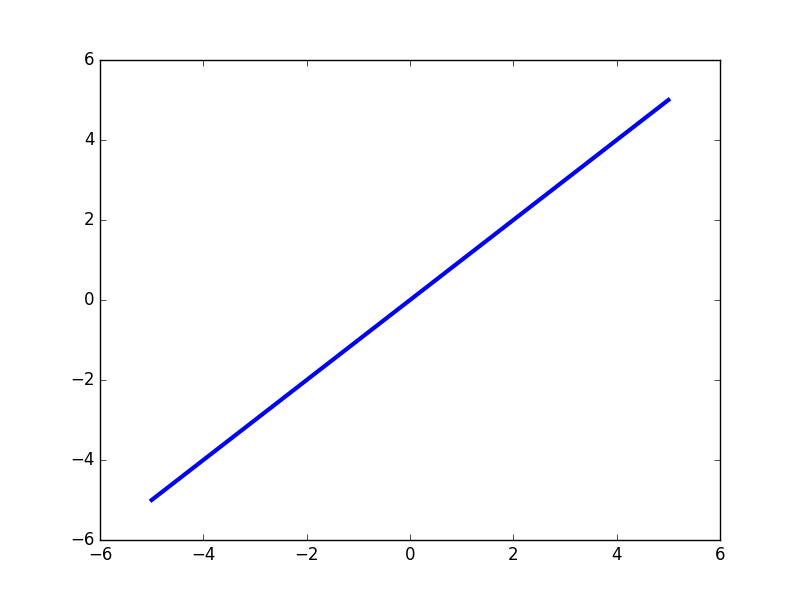
\includegraphics[scale=0.25]{images/chapter1/id.png} & 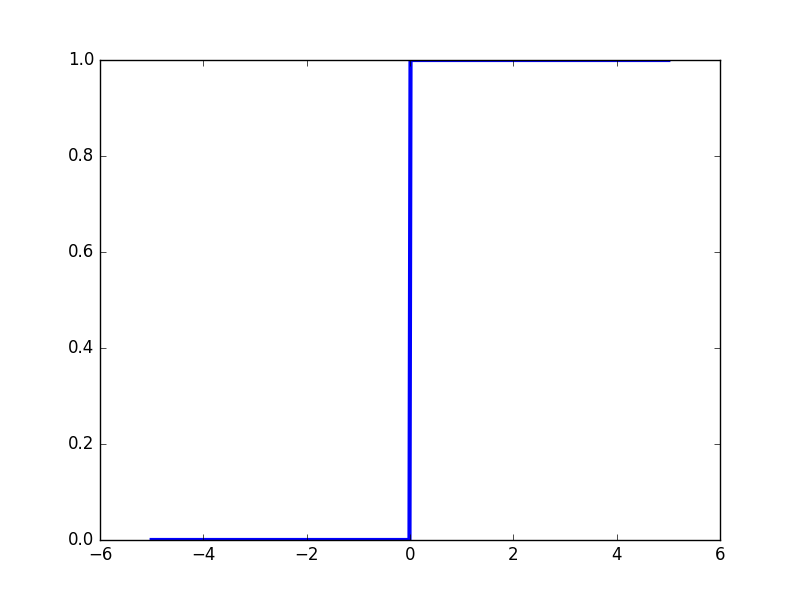
\includegraphics[scale=0.25]{images/chapter1/u.png} \\
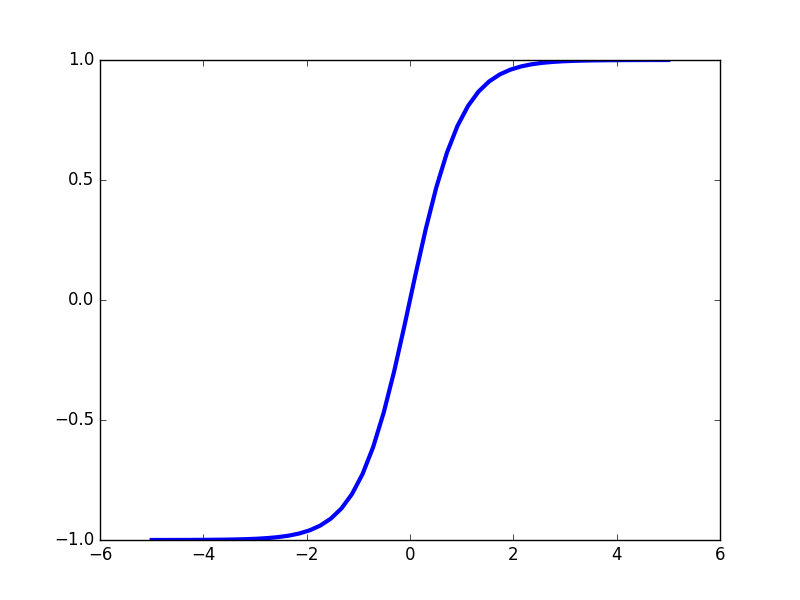
\includegraphics[scale=0.25]{images/chapter1/tanh.png} & 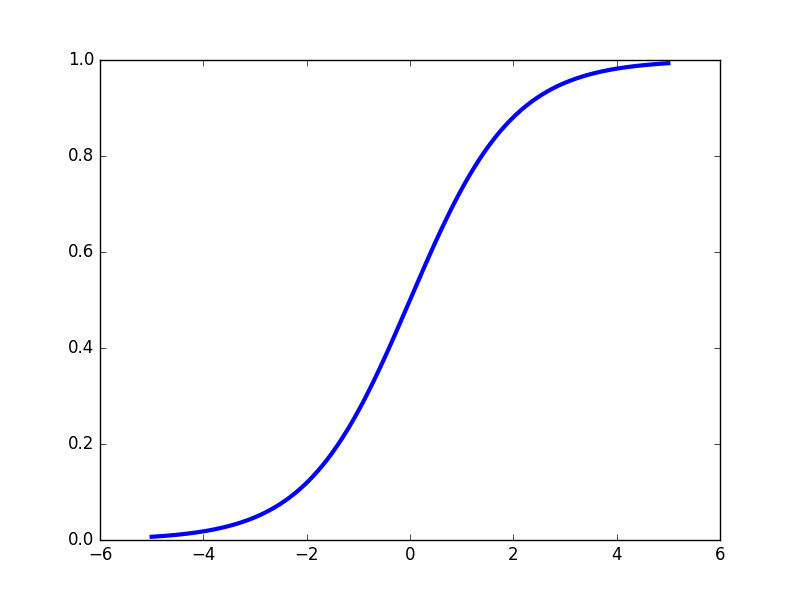
\includegraphics[scale=0.25]{images/chapter1/s.png} \\
\multicolumn{2}{c}{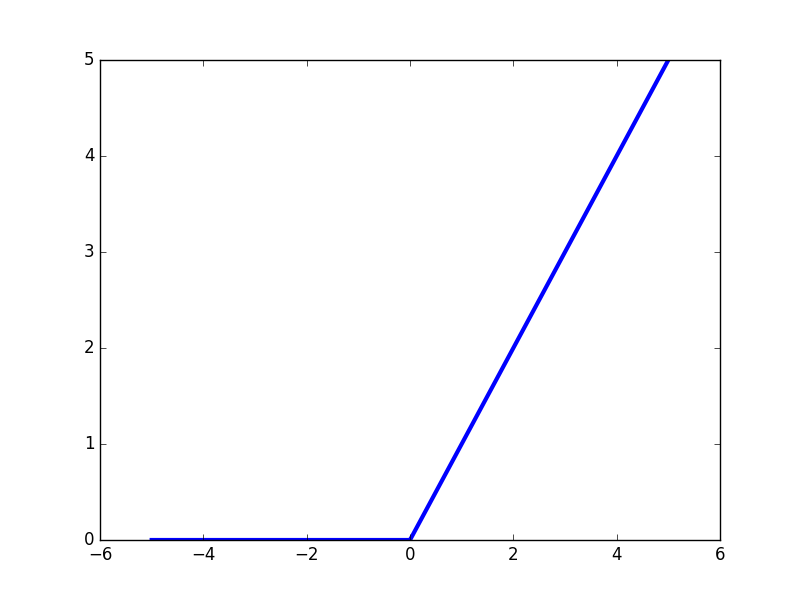
\includegraphics[scale=0.25]{images/chapter1/relu.png}}
\end{tabular}
\caption{Graphe entre -5 et 5 de la fonction identité (en haut à gauche), de l'échelon (en haut à droite), de la tangente hyperbolique (au milieu à gauche), de la sigmoïde (au milieu à droite) et de ReLU (en bas).} 
\label{fonctions_activation}
\end{center}
\end{figure}

Il est possible de se servir d'un neurone seul pour résoudre des problèmes de classification ou de régression. Détaillons quelques exemples importants.

\medbreak

\begin{example}[Perceptron]
Un neurone avec comme fonction d'activation un échelon sépare l'espace en deux par un hyperplan de vecteur normal $w$. En effet :

\begin{itemize}
\item $ \forall x \in \mathbb{R}^n, w^Tx < 0 \Rightarrow f(x) = 0$
\item $ \forall x \in \mathbb{R}^n w^Tx \geq 0 \Rightarrow f(x) = 1$
\end{itemize}

La figure \ref{hyperplan} illustre cette séparation. Ce cas particulier de neurone est couramment appelé perceptron.
\end{example}

\begin{figure}
\begin{center}
\pagestyle{empty}
\definecolor{qqqqff}{rgb}{0,0,1}
\definecolor{ffqqqq}{rgb}{1,0,0}
\begin{tikzpicture}[line cap=round,line join=round,>=triangle 45,x=1.0cm,y=1.0cm]
\draw[->,color=black] (-5.42,0) -- (5.45,0);
\foreach \x in {-5,-4,-3,-2,-1,1,2,3,4,5}
\draw[shift={(\x,0)},color=black] (0pt,2pt) -- (0pt,-2pt) node[below] {\footnotesize $\x$};
\draw[->,color=black] (0,-2.99) -- (0,5.07);
\foreach \y in {-2,-1,1,2,3,4,5}
\draw[shift={(0,\y)},color=black] (2pt,0pt) -- (-2pt,0pt) node[left] {\footnotesize $\y$};
\draw[color=black] (0pt,-10pt) node[right] {\footnotesize $0$};
\clip(-5.42,-2.99) rectangle (5.45,5.07);
\fill[line width=0pt,color=ffqqqq,fill=ffqqqq,fill opacity=0.1] (-12.7,-3.03) -- (15.5,5.76) -- (10.12,27.67) -- (-20,20) -- cycle;
\fill[line width=0pt,color=qqqqff,fill=qqqqff,fill opacity=0.1] (-12.7,-3.03) -- (-3.47,-28.78) -- (29.71,-17.95) -- (15.5,5.76) -- cycle;
\draw [domain=-5.42:5.45] plot(\x,{(-1.14-0.38*\x)/-1.22});
\draw [->] (1.12,1.28) -- (0.74,2.5);
\draw (0.74,2.89) node[anchor=north west] {$ w $};
\end{tikzpicture}
\caption{Hyperplan séparateur dans un espace à deux dimensions correspondant à un certain vecteur de poids $w$. La partie rouge correspond aux entrées classifiées 1 et en bleue celles qui sont classifiées 0.}
\label{hyperplan}
\end{center}
\end{figure}

\vspace{1cm}

\begin{example}[Régression logistique]
Si la fonction d'activation est une sigmoïde, la sortie du neurone peut être interprétée comme la probabilité $p(y=1|x)$. Par conséquent, le neurone classifie un exemple dans la classe 1 si la sortie est supérieure à $0.5$ et dans la classe 0 sinon. On parle ici de régression logistique. L'espace est toujours séparé en deux parties par un hyperplan, $H = \{x, f(x)=0.5\}$. Cependant les valeurs associées aux entrées sont désormais continues entre $0$ et $1$. La figure \ref{regression_logistique} permet de visualiser cette différence. Dans la suite de ce document, des graphes de ce type seront utilisés à plusieurs reprises afin de pouvoir visualiser l'action d'un réseau de neurones.
\end{example}

\begin{figure}[H]
\begin{center}
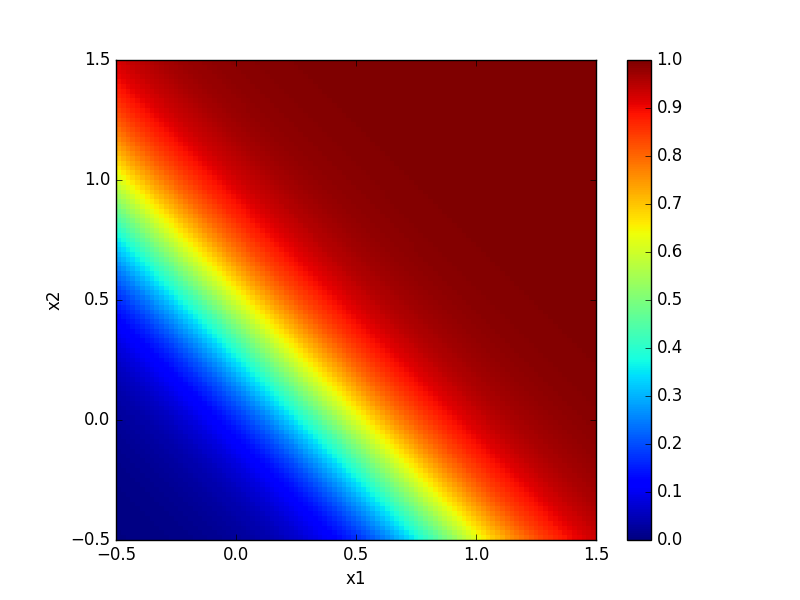
\includegraphics[scale=0.5]{images/chapter1/or.png}
\caption{Sortie d'une régression logistique prenant en entrée un vecteur de $\mathbb{R}^2$ sur $[-0.5, 1.5] \times [-0.5, 1.5]$. L'axe $x_1$ et l'axe $x_2$ correspondent respectivement à la première et à la deuxième coordonnée de l'entrée.}
\label{regression_logistique}
\end{center}
\end{figure}

\begin{example}[Régression linéaire]
Finalement, si la fonction d'activation est la fonction identité, le neurone sera capable d'atteindre toutes les valeurs réelles. Il pourra donc résoudre un problème de régression. Il s'agit de la régression linéaire.
\end{example}

Le point commun entre tous les neurones est qu'ils sont seulement capables de modéliser des interactions linéaires entre les entrées. Cependant, à partir d'un ensemble de données, il est possible d'utiliser des neurones pour modéliser des interactions non linéaires entre les différentes composantes des entrées. Pour cela, il faut transformer les entrées afin de créer de nouvelles composantes. Par exemple, prenons un ensemble de données tel que les points ont le label $1$ s'ils sont dans le disque de rayon 0.5 et de centre $(0;0)$ et $0$ sinon. Un exemple d'un tel ensemble de données est visible sur la figure \ref{disque}. En l'état, cet ensemble n'est pas linéairement séparable et donc un neurone simple ne peut pas le classifier correctement. Cependant si une transformation telle que $x \mapsto (x_1, x_2, x_1x_2, x_1^2, x_2^2)$ est appliquée aux exemples, les points sont alors linéairement séparables dans ce nouvel espace. Il est alors possible d'utiliser un neurone afin de classifier correctement l'ensemble. Ces résultats sont présents sur la figure \ref{disque}.

\begin{figure}[H]
\begin{center}
\begin{tabular}{cc}
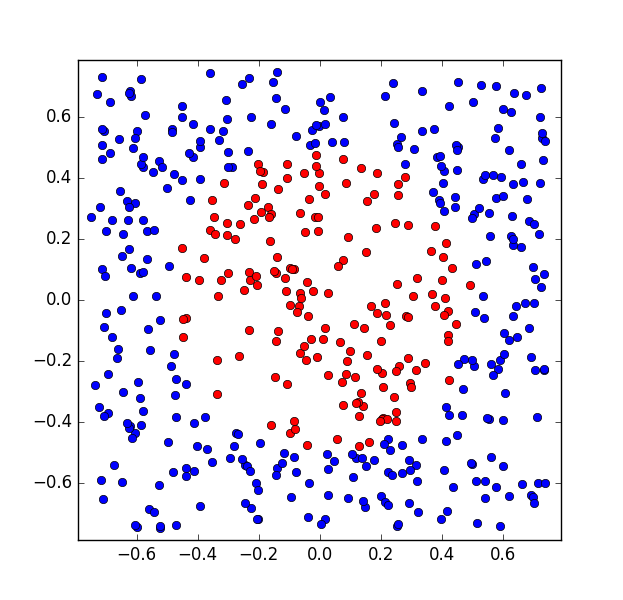
\includegraphics[scale=0.35]{images/chapter1/disk_dataset.png} & 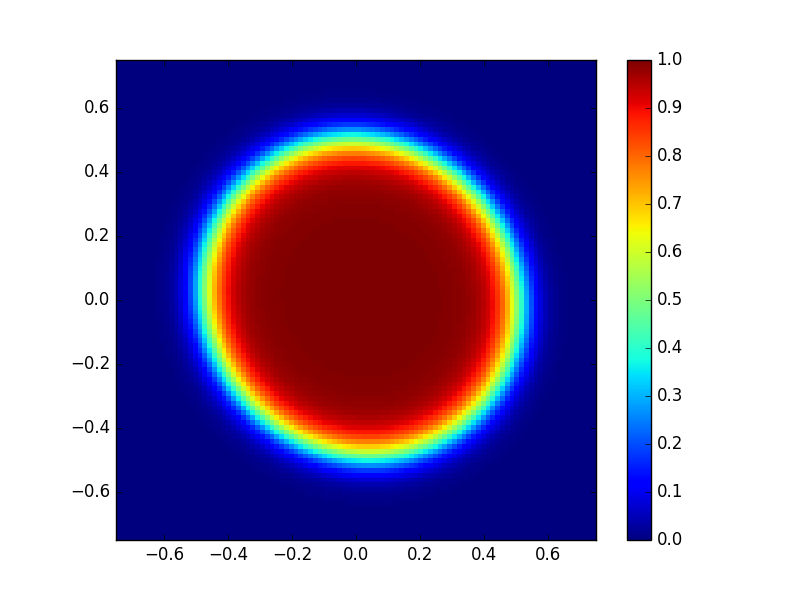
\includegraphics[scale=0.35]{images/chapter1/disk_learned.png} \\
\end{tabular}
\caption{À gauche un ensemble de données de 500 points. Les points à l'intérieur du cercle de rayon 0.5 et de centre $(0; 0)$ sont en rouge, les autres en bleu. À droite, la représentation du disque apprise par le neurone.} 
\label{disque}
\end{center}
\end{figure}

En conclusion, un neurone est une fonction relativement simple permettant de modéliser des interactions linéaires entre ses entrées. Dans la partie suivante, nous verrons comment associer ces neurones afin de créer des modèles plus complexes.

\section{Un réseau de neurones}

\begin{definition}[Réseau de neurones]
Un réseau de neurones est défini par un graphe orienté $\mathcal{G}(V, A)$ où les n\oe{}uds sont des neurones et les arêtes des liens entre les neurones et par un ensemble de neurones d'entrée $V_{in} \subset V$ et de neurones de sorties $V_{out} \subset V$. Une arête partant d'un neurone $i$ vers un neurone $j$ signifie que la sortie du neurone $i$ est une entrée pour le neurone $j$. Notons $f_{j}$ la fonction représentant le neurone $j$. Finalement, nous noterons un réseau $\mathcal{N}(V, A, V_{in}, V_{out}, f)$ où $f$ est l'ensemble des fonctions des neurones.
\end{definition}

Si nous notons $\{i \text{ tel que } (i, j) \in A\}$ l'ensemble des indices des parents du neurone $j$ et $\{j \text{ tel que } (i, j) \in A\}$ l'ensemble des indices des enfants du neurone $i$. Alors la sortie du neurone $j$ est :

\begin{equation}
y_{j} = f_{j}((y_{i})_{i \text{ tel que } (i, j) \in A})
\label{eq_propagation}
\end{equation} 

Il existe certaines classes particulières de réseau de neurones. Tout d'abord, s'il contient des cycles, il sera dit récurrent. Dans le cas contraire, on parlera de réseau \textit{feedforward}. Puis, s'il est possible de l'organiser sous forme de couches où les sorties des neurones d'une couche sont les entrées de la couche suivante, on parle de réseau de neurones multicouche dit aussi MLP (multilayer perceptron). Des exemples des différents types de réseaux sont présents sur la figure \ref{reseaux}.

\begin{figure}
\begin{center}
\begin{tabular}{cc}
\begin{tikzpicture}[scale=0.30][line cap=round,line join=round,>=triangle 45,x=1.0cm,y=1.0cm]
\clip(-3.5,-5.5) rectangle (13.5,7);
\draw(-1,4) circle (1cm);
\draw(-1,1) circle (1cm);
\draw(-1,-2) circle (1cm);
\draw(3,3) circle (1cm);
\draw(3,-1) circle (1cm);
\draw(7,3) circle (1cm);
\draw(11,3) circle (1cm);
\draw(11,-1) circle (1cm);
\draw [->] (0,4) -- (2,3);
\draw [->] (0,1) -- (2,3);
\draw [->] (0,-2) -- (2,-1);
\draw [->] (0,1) -- (2,-1);
\draw [->] (3,0) -- (3,2);
\draw(7,-1) circle (1cm);
\draw [->] (7,2) -- (4,-1);
\draw [->] (4,3) -- (6,3);
\draw [->] (4,-1) -- (6,-1);
\draw [->] (7,0) -- (7,2);
\draw [->] (8,3) -- (10,3);
\draw [->] (8,-1) -- (10,-1);
\draw [rotate around={90:(-1,1)},dash pattern=on 3pt off 3pt] (-1,1) ellipse (5.22cm and 1.5cm);
\draw (-3.5,-4.15) node[anchor=north west] {$ Entrées $};
\draw [rotate around={90:(11,1)},dash pattern=on 3pt off 3pt] (11,1) ellipse (4.25cm and 1.45cm);
\draw (8.8,-3.21) node[anchor=north west] {$ Sorties $};
\draw (-1.7,4.6) node[anchor=north west] {$ 1 $};
\draw (-1.95,1.6) node[anchor=north west] {$ x_1 $};
\draw (-1.95,-1.4) node[anchor=north west] {$ x_2 $};
\draw (2.1,3.9) node[anchor=north west] {$ f_1 $};
\draw (2.1,-0.1) node[anchor=north west] {$ f_2 $};
\draw (6,3.9) node[anchor=north west] {$ f_3 $};
\draw (6,-0.1) node[anchor=north west] {$ f_4 $};
\draw (10,3.7) node[anchor=north west] {$ y_1 $};
\draw (10,-0.3) node[anchor=north west] {$ y_2 $};
\end{tikzpicture} & 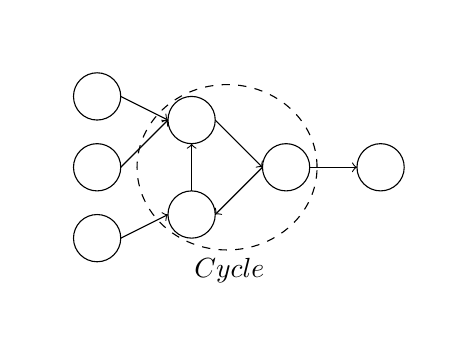
\begin{tikzpicture}[scale=0.3][line cap=round,line join=round,>=triangle 45,x=1.0cm,y=1.0cm]
\clip(-3.94,-7.74) rectangle (13.14,4.91);
\draw(-1,2) circle (1cm);
\draw(-1,-1) circle (1cm);
\draw(-1,-4) circle (1cm);
\draw(3,1) circle (1cm);
\draw(3,-3) circle (1cm);
\draw(7,-1) circle (1cm);
\draw(11,-1) circle (1cm);
\draw [->] (0,2) -- (2,1);
\draw [->] (0,-1) -- (2,1);
\draw [->] (0,-4) -- (2,-3);
\draw [->] (4,1) -- (6,-1);
\draw [->] (3,-2) -- (3,0);
\draw [->] (6,-1) -- (4,-3);
\draw [->] (8,-1) -- (10,-1);
\draw [rotate around={0:(4.5,-1)},dash pattern=on 3pt off 3pt] (4.5,-1) ellipse (3.81cm and 3.5cm);
\draw (2.7,-4.43) node[anchor=north west] {$ Cycle $};
\end{tikzpicture} \\
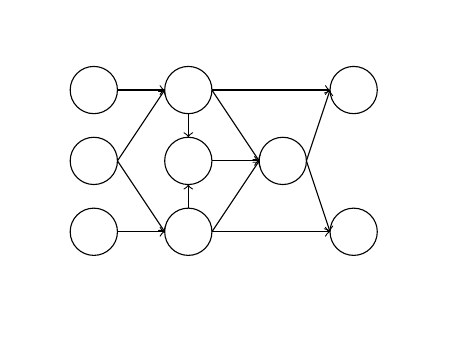
\begin{tikzpicture}[scale=0.3][line cap=round,line join=round,>=triangle 45,x=1.0cm,y=1.0cm]
\clip(-3.8,-5.74) rectangle (12.92,6.64);
\draw(-1,1) circle (1cm);
\draw(-1,4) circle (1cm);
\draw(-1,-2) circle (1cm);
\draw(3,4) circle (1cm);
\draw(3,-2) circle (1cm);
\draw(3,1) circle (1cm);
\draw(7,1) circle (1cm);
\draw(10,4) circle (1cm);
\draw(10,-2) circle (1cm);
\draw [->] (0,4) -- (2,4);
\draw [->] (0,1) -- (2,4);
\draw [->] (0,1) -- (2,-2);
\draw [->] (0,-2) -- (2,-2);
\draw [->] (3,-1) -- (3,0);
\draw [->] (3,3) -- (3,2);
\draw [->] (4,1) -- (6,1);
\draw [->] (4,-2) -- (6,1);
\draw [->] (4,4) -- (6,1);
\draw [->] (8,1) -- (9,4);
\draw [->] (8,1) -- (9,-2);
\draw [->] (4,-2) -- (9,-2);
\draw [->] (4,4) -- (9,4);
\end{tikzpicture} & 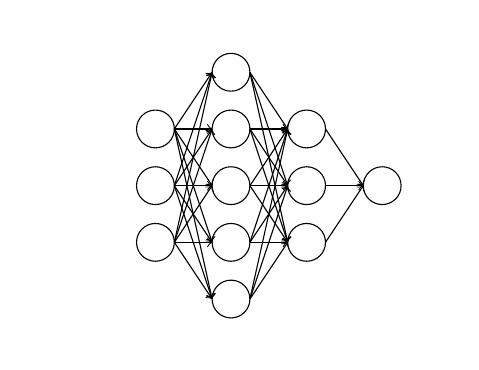
\begin{tikzpicture}[scale=0.24][line cap=round,line join=round,>=triangle 45,x=1.0cm,y=1.0cm]
\clip(-8.76,-5.24) rectangle (13.65,11.36);
\draw(-2,6) circle (1cm);
\draw(-2,3) circle (1cm);
\draw(-2,0) circle (1cm);
\draw(2,3) circle (1cm);
\draw(2,6) circle (1cm);
\draw(2,0) circle (1cm);
\draw(2,-3) circle (1cm);
\draw(2,9) circle (1cm);
\draw(6,6) circle (1cm);
\draw(6,3) circle (1cm);
\draw(6,0) circle (1cm);
\draw(10,3) circle (1cm);
\draw [->] (-1,6) -- (1,9);
\draw [->] (-1,6) -- (1,6);
\draw [->] (-1,6) -- (1,3);
\draw [->] (-1,6) -- (1,0);
\draw [->] (-1,3) -- (1,9);
\draw [->] (-1,3) -- (1,6);
\draw [->] (-1,3) -- (1,3);
\draw [->] (-1,3) -- (1,0);
\draw [->] (-1,0) -- (1,0);
\draw [->] (-1,0) -- (1,3);
\draw [->] (-1,0) -- (1,6);
\draw [->] (-1,0) -- (1,9);
\draw [->] (3,9) -- (5,6);
\draw [->] (3,6) -- (5,6);
\draw [->] (3,3) -- (5,6);
\draw [->] (3,0) -- (5,6);
\draw [->] (3,6) -- (5,3);
\draw [->] (3,3) -- (5,3);
\draw [->] (3,3) -- (5,0);
\draw [->] (3,9) -- (5,3);
\draw [->] (3,9) -- (5,0);
\draw [->] (3,6) -- (5,0);
\draw [->] (3,0) -- (5,0);
\draw [->] (3,0) -- (5,3);
\draw [->] (-1,6) -- (1,-3);
\draw [->] (-1,3) -- (1,-3);
\draw [->] (-1,0) -- (1,-3);
\draw [->] (3,-3) -- (5,0);
\draw [->] (3,-3) -- (5,3);
\draw [->] (3,-3) -- (5,6);
\draw [->] (7,6) -- (9,3);
\draw [->] (7,3) -- (9,3);
\draw [->] (7,0) -- (9,3);
\end{tikzpicture} \\
\end{tabular}
\caption{Exemples de réseaux de neurones. Un réseau de neurones quelconque (en haut à gauche),  récurrent (en haut à droite), feedforward (en bas à gauche) et multicouche (en bas à droite).} 
\label{reseaux}
\end{center}
\end{figure}

Dans les sections suivantes seront étudiés les algorithmes pour évaluer la sortie d'un réseau de neurones puis pour l’entraîner. Nous nous limiterons aux algorithmes d'entrainement des réseaux de neurones feedforward. Les algorithmes concernant les réseaux de neurones récurrent seront abordés dans le \autoref{chap:Réseaux de neurones récurrents}.

\section{Propagation}

L'algorithme de propagation dans le cadre des réseaux feedforward est très simple. Il suffit de mettre à jour les neurones d'entrée puis d'appliquer la formule \ref{eq_propagation} récursivement en partant des neurones dans $V_{out}$.

Ainsi, un premier algorithme naïf est :

\begin{algorithm}[H]
\begin{algorithmic}
\Procedure{$evaluer\_reseau$}{$\mathcal{N}(V, A, V_{in}, V_{out}, f), x$}
\Function{$evaluer\_neurone$}{$j$}
	\If{$j \in V_{in}$}
    	\State \Return $x_j$
	\Else
		\State $t \leftarrow (evaluer\_neurone(i), i \text{ tel que } (i, j) \in A)$
		\State \Return $f_j(t)$
	\EndIf
\EndFunction

\For{$j \in V_{out}$}
	\State $y_j \leftarrow evaluer\_neurone(j)$ 
\EndFor
\EndProcedure
\end{algorithmic} 
\caption{Algorithme naïf d'évaluation d'un réseau de neurones feedforward. Il prend en entrée un réseau de neurones et un vecteur d'entrée pour le réseau.}
\end{algorithm}

Cette version n'est pas du tout efficace, elle calcule plusieurs fois la sortie de chaque neurone. Si le graphe est densément connecté, l'algorithme aura un coût temporel extrêmement élevé. Une amélioration simple consiste à rajouter de la mémoïsation afin de garantir que la sortie de chaque neurone sera calculée au plus une fois. Le pseudo-code de cet algorithme correspond à l'algorithme \ref{mem}.

\begin{algorithm}[H]
\begin{algorithmic}
\Procedure{$evaluer\_reseau$}{$\mathcal{N}(V, A, V_{in}, V_{out}, f), x$}
\Function{$evaluer\_neurone$}{$j$}
	\If{$déjàCalculé[j]$ est $faux$}
		\State $t \leftarrow (evaluer\_neurone(i), i \text{ tel que } (i, j) \in A)$
		\State $y_j \leftarrow f_j(t)$
		\State $déjàCalculé[j] \leftarrow vrai$
	\EndIf
	\State \Return $y_j$
\EndFunction

\State Initialiser un tableau $dejaCalculé$ de longueur $|V|$ à $faux$.
\For{$i \in V_{in}$}
	\State $y_i \leftarrow x_i$
	\State $déjàCalculé[i] \leftarrow vrai$ 
\EndFor
\For{$j \in V_{out}$}
	\State $evaluer\_neurone(j)$ 
\EndFor
\EndProcedure
\end{algorithmic}
\caption{Algorithme d'évaluation d'un réseau de neurones feedforward utilisant la mémoïsation afin de ne pas recalculer plusieurs fois la sortie d'un neurone.}
\label{mem}
\end{algorithm}

Cet algorithme calcule au plus une fois la sortie de chaque neurone et il appelle $evaluer\_neurone$ au plus $|A|$ fois, il a donc un coût temporel en $O(|V|+|A|)$. Ce qui est a priori le coût optimal.

\section{Fonctions de coût}

Avant de parler des algorithmes d'apprentissage et de la manière de modifier les poids avant d'approcher une fonction, nous allons revenir sur les fonctions de coût. Dans la suite, nous justifierons l'utilisation et le bien-fondé des fonctions de coût les plus courantes.

Il sera détaillé trois fonctions de coût : une pour la régression, une pour la classification binaire et une pour la classification à plusieurs classes. La même méthode sera utilisée à chaque fois : un modèle sera proposé puis la fonction de coût sera déduite en utilisant le principe du maximum de vraisemblance.

\begin{definition}[Fonction de vraisemblance]
Si $x_1, ..., x_n$ sont des échantillons générés indépendamment par une probabilité $p_{\theta}$ la vraisemblance de l'échantillon est alors :
$$
L(\theta) = \prod_{i=1}^{N}{p_{\theta}(x^{(i)})}
$$
\end{definition}

\begin{remark}
Dans notre cas, les échantillons $(x_1, y_1), ..., (x_n, y_n)$ sont générés par la loi $p_{\theta}(y|x)$ où $\theta$ sont les paramètres du modèle, la vraisemblance est donc :
$$
L(\theta) = \prod_{i=1}^{N}{p_{\theta}(y^{(i)}|x^{(i)})}
$$
\end{remark}

\begin{definition}[Maximum de vraisemblance]
Le paramètre $\theta$ maximise la vraisemblance si $\theta \in argmax L(\theta')$.
\end{definition}

\begin{remark}
Maximiser la vraisemblance revient donc à rechercher le maximum d'une fonction.
\end{remark}

\begin{remark}
Au lieu de maximiser la vraisemblance, nous allons minimiser l'opposé du logarithme de la vraisemblance (\textit{negative log-likelihood} en anglais). On obtient alors :
\begin{equation}
NLL(\theta) = -\sum_{i=1}^{N}{\log{p_{\theta}(y^{(i)}|x^{(i)})}}
\label{NLL}
\end{equation}
Cette forme est préférée car la somme est plus facile à dériver que le produit. En outre, l'opposé du logarithme de la vraisemblance est pris pour se ramener à un problème de minimisation.
\end{remark}

\subsection{Régression}

Dans un problème de régression, il est courant de choisir comme modèle :

\begin{equation}
p_{\theta}(y|x) \sim \mathcal{N}(\hat{y}(x, \theta), \sigma) \Leftrightarrow p_{\theta}(y|x) = \frac{1}{\sqrt{2\pi}\sigma}\exp{(\frac{-(y - \hat{y})^2}{2\sigma^2})}
\label{modele_normale}
\end{equation}

Où $\theta$ est l'ensemble des poids de notre réseau, $\hat{y}(x, \theta)$ est la sortie de notre réseau quand l'entrée est $x$ et $\sigma$ une constante positive. On se permettra de noter seulement $\hat{y}(x)$ au lieu de $\hat{y}(x, \theta)$ pour plus de légèreté.


En remplaçant $p_{\theta}$ par l'expression \ref{modele_normale} dans l'équation \ref{NLL}, on obtient :

\begin{equation}
NLL(\theta) = \sum_{i=1}^{N}{(y^{(i)} - \hat{y}(x^{(i)}))^2} + C
\end{equation}

où $C$ est une constante.

Dans le problème de minimisation, la constante peut être négligée et il est possible de multiplier par une constante positive sans changer le problème. On déduit que sous cette modélisation, une fonction de coût obtenue par le principe de maximum de vraisemblance est :

\begin{equation}
E = \frac{1}{N}\sum_{i=1}^{N}{(y^{(i)} - \hat{y}(x^{(i)}))^2} = \frac{1}{N}\sum_{i=1}^{N}{e(y^{(i)}, \hat{y}(x^{(i)}))}
\end{equation}

avec $e : (x, y) \mapsto (x - y)^2$. Cette fonction est appelée erreur quadratique moyenne (\textit{mean squared error} en anglais).

\subsection{Classification binaire}

Dans le cas de la classification binaire, à $x$ fixé, $p(y|x)$ suit une loi de Bernoulli. Un modèle possible est donc :

\begin{equation}
p_{\theta}(y|x) \sim \mathcal{B}(\hat{y}(x, \theta)) \Leftrightarrow p_{\theta}(y|x) = 
\left\{
    \begin{array}{ll}
        \hat{y}(x) \text{ si } y = 1 \\
        1 - \hat{y}(x) \text{ sinon}
    \end{array}
\right.
\label{modele_bernoulli}
\end{equation}

La formule \ref{modele_bernoulli} peut se réécrire de manière plus compacte :
\begin{equation}
p_{\theta}(y|x) = \hat{y}(x)^y(1-\hat{y}(x))^{1-y}
\label{modele_bernoulli_compact}
\end{equation}

En utilisant cette dernière forme, on obtient que l'expression de la \textit{negative log-likelihood} est : 

\begin{equation}
NLL(\theta) = -\sum_{i=1}^{N}{y^{(i)}\log\hat{y}(x^{(i)})+(1-y^{(i)})\log(1-\hat{y}(x^{(i)}))}
\end{equation}

On en déduit de même que précédemment que notre fonction de coût est :

\begin{equation}
E = \frac{1}{N}\sum_{i=1}^{N}{-(y^{(i)}\log\hat{y}(x^{(i)})+(1-y^{(i)})\log(1-\hat{y}(x^{(i)})))} = \frac{1}{N}\sum_{i=1}^{N}{e(y^{(i)}, \hat{y}(x^{(i)}))}
\end{equation}

avec $e : (x, y) \mapsto -(x \log y + (1-x)\log(1-y))$.

\subsection{Classification à plusieurs classes}

Finalement, dans le cas d'une classification à plusieurs classes, $p(y|x)$ est une loi Multinoulli à $x$ fixé. Si la sortie $\hat{y}$ du réseau est un vecteur de longueur $M$ avec $M$ le nombre de classes, une sortie possible est :

\begin{equation}
p_{\theta}(y|x) \sim \mathcal{M}(\hat{y}(x, \theta)_0, ..., \hat{y}(x, \theta)_{M-1}) \Leftrightarrow p_{\theta}(y|x) = \hat{y}(x)_y
\label{modele_multinoulli}
\end{equation}

La \textit{negative log-likelihood} associée est donc :

\begin{equation}
NLL(\theta) = -\sum_{i=1}^{N}{\log \hat{y}(x^{(i)})_{y^{(i)}}}
\label{NLL_multinoulli}
\end{equation}

Posons pour tout $i \in \{0, ..., M-1\}$, $\tau^{(i)} \in \mathbb{R}^M$ le vecteur tel que :

$$ \tau^{(i)}_j = 
\left\{
    \begin{array}{ll}
        1 \text{ si } i = j \\
        0 \text{ sinon}
    \end{array}
\right.
$$

Il est alors possible de réécrire la formule \ref{NLL_multinoulli} en utilisant ces vecteurs :

\begin{equation}
NLL(\theta) = \sum_{i=1}^{N}{-\sum_{j=0}^{M-1}{\tau^{(y^{(i)})}_j\log \hat{y}(x^{(i)})_j}}
\end{equation}

Enfin en introduisant l'entropie croisée $H$ définie de manière générale par :

$$
H(p, q) = -\sum_{x}{p(x)\log q(x)}
$$

On obtient que :

\begin{equation}
NLL(\theta) = \sum_{i=1}^{N}{H(\tau^{(y^{(i)})}, \hat{y}(x^{(i)}))}
\end{equation}

On a remplacé $y$ par un vecteur nul possédant un $1$ à la position $y$, une telle transformation est couramment appelé encodage \textit{one-hot}. 

Notre fonction de coût sera donc :

\begin{equation}
E = \frac{1}{N}\sum_{i=1}^{N}{H(\tau^{(y^{(i)})}, \hat{y}(x^{(i)}))} = \frac{1}{N}\sum_{i=1}^{N}{e(y^{(i)}, \hat{y}(x^{(i)}))}
\end{equation}

Avec $e : (x, y) \mapsto H(\tau^x, y)$. Cette fonction de coût est naturellement appelée entropie croisée (\textit{cross-entropy} en anglais).

\section{Descente du gradient}

Étant donné une fonction de coût $E$, l'objectif de l'apprentissage est de déterminer les poids permettant de minimiser $E$. Dans l'idéal, il faudrait pouvoir exprimer $E$ en fonction des poids, dériver $E$ par rapport à chaque poids puis chercher les valeurs des poids atteignant les minima. Malheureusement, dans la plupart des cas, il est impossible d'avoir de telles solutions analytiques.

Une solution à ce problème est la descente du gradient, un procédé itératif consistant à modifier légèrement les valeurs des poids afin qu'à chaque étape $E$ décroisse.  En notant, $\theta$ le vecteur contenant les poids de tous les neurones du réseau, la valeur de ces poids changera à chaque itération, par conséquent, notons $\theta(t)$ la valeur de $\theta$ à l'itération $t$. La direction selon laquelle $E$ augmente le plus est $\frac{\partial E}{\partial \theta}$, la direction selon laquelle $E$ décroît le plus est donc $-\frac{\partial E}{\partial \theta}$. Si les poids sont modifiés en se déplaçant dans cette direction d'un pas $\eta(t)$ assez petit, le coût diminuera. L'équation d'évolution est donnée par \ref{mise_a_jour_poids}.

\begin{equation}
\theta(t+1) = \theta(t) - \eta(t) \frac{\partial E}{\partial \theta}
\label{mise_a_jour_poids}
\end{equation}

Il existe plusieurs stratégies afin de choisir le pas $\eta(t)$. Dans un premier temps et pour plus de simplicité, nous choisirons un pas $\eta(t)=\eta$ constant.

\section{Rétropropagation du gradient}

L'application de l'algorithme précédant nécessite le calcul des dérivées partielles par rapport à chacun des poids du réseau de neurones. Prenons le neurone $j$ du réseau. Son entrée est notée $x_j$, sa sortie $y_j$, sa fonction d'activation $g_j$ et ses poids $w_j$. De plus, définissons la quantité intermédiaire $s_j = w_j^Tx_j$. La formule \ref{sortie_neurone2} appliquée à ce neurone est donc $y_j = g_j(w_j^Tx_j) = g(s_j)$. En utilisant la règle de la chaîne, on obtient :

\begin{equation}
\frac{\partial E}{\partial w_j} = \frac{\partial E}{\partial y_j}\frac{\partial y_j}{\partial s_j}\frac{\partial s_j}{\partial w_j}
\label{dEdw_avant}
\end{equation}

On peut remarquer que le terme $\frac{\partial s_j}{\partial w_j}$ est égal à $x_j$ et que $\frac{\partial y_j}{\partial s_j} = g'(s_j)$ d'où l'égalité \ref{dEdw_avant} devient :

\begin{equation}
\frac{\partial E}{\partial w_j} = \frac{\partial E}{\partial y_j} g_j'(s_j) x_j
\label{dEdw}
\end{equation}

Afin de calculer $\frac{\partial E}{\partial y_j}$, utilisons le fait que la sortie du neurone $j$ est une des entrées de ses enfants. En notant $x_{i, j}$ l'entrée du neurone $i$ correspondant à la sortie du neurone $j$, on a :

\begin{equation}
\frac{\partial E}{\partial y_j} = \sum_{i \text{ tel que } (j, i) \in A}{\frac{\partial E}{\partial x_{i,j}}}
\label{formule_retropropagation}
\end{equation}

La formule \ref{formule_retropropagation} montre que si on calcule $\frac{\partial E}{\partial x_i}$, la dérivée du coût par rapport aux entrées d'un neurone, il est aisé de calculer la dérivée du coût par rapport aux poids pour les parents de ce neurone. Or la dérivée du coût par rapport aux entrées d'un neurone est facilement calculable en utilisant l'égalité suivante :

\begin{equation}
\frac{\partial E}{\partial x_j} = \frac{\partial E}{\partial y_j}\frac{\partial y_j}{\partial s_j}\frac{\partial s_j}{\partial x_j} =  \frac{\partial E}{\partial y_j} g_j'(s_j) w_j
\label{dEdx}
\end{equation}

Finalement, en utilisant les formules \ref{dEdw}, \ref{formule_retropropagation} et \ref{dEdx}, il est possible de rétropropager le gradient et de calculer $\frac{\partial E}{\partial w_j}$ pour tout neurone $j$. On en déduit l'algorithme suivant :

\begin{algorithm}[H]
\begin{algorithmic}
\Procedure{$retropropager\_gradient$}{$\mathcal{N}(V, A, V_{in}, V_{out}, f), x, y$}
\Function{$calculer\_gradient$}{$j$}
	\If{$déjàCalculé_j$ est $faux$}
		\State $\frac{\partial E}{\partial y_j} \leftarrow \sum_{i \text{ tel que } (j, i) \in A}{calculer\_gradient(i)_j}$
		\State $\frac{\partial E}{\partial x_j} \leftarrow \frac{\partial E}{\partial y_j} g_j'(s_j) w_j$
		\State $\frac{\partial E}{\partial w_j} \leftarrow \frac{\partial E}{\partial y_j} g_j'(s_j) x_j$
		\State $déjàCalculé_j \leftarrow vrai$
	\EndIf
	\State \Return $\frac{\partial E}{\partial x_j}$
\EndFunction

\State Appeler $evaluer\_reseau(\mathcal{N}(V, A, V_{in}, V_{out}, f), x)$ et récupérer les entrées et sorties de chaque neurone
\State Initialiser un tableau $dejaCalculé$ de longueur $|V|$ à $faux$.
\For{$i \in V_{out}$}
	\State Calculer $\frac{\partial E}{\partial y_i}$
	\State $déjàCalculé_i \leftarrow vrai$ 
\EndFor
\For{$i \in V$}
	\State $calculer\_gradient(i)$ 
\EndFor
\EndProcedure
\end{algorithmic} 
\caption{Algorithme de rétropropagation du gradient dans un réseau de neurone feedforward.}
\label{propagation_memoisation2}
\end{algorithm}

Cet algorithme utilise la mémoïsation afin de ne pas calculer plusieurs fois les dérivées pour un neurone. On peut remarquer que cet algorithme est très similaire à celui de la propagation. Pour des raisons similaires, le coût temporel de la rétropropagation est aussi en $O(|V|+|A|)$.